%% main.tex
%% Asimov Cascade Monitoring in Humanoid Robotics -- v2.5 manuscript
%% Content-faithful port of the Word draft (draft_raw.tex); IEEEconf format

\documentclass[letterpaper,9pt,conference]{ieeeconf}

\IEEEoverridecommandlockouts
\overrideIEEEmargins

\usepackage{cite}
\usepackage{amsmath,amssymb,amsfonts}
\usepackage{graphicx}
\graphicspath{{./figures/}}
\usepackage{array}
\usepackage{tabularx}
\usepackage{booktabs}
\usepackage[table]{xcolor}
\usepackage{stfloats}
\usepackage{ulem}
\usepackage[colorlinks=true,linkcolor=black,citecolor=black,urlcolor=blue]{hyperref}

\makeatletter
\newcommand{\linebreakand}{\end{@IEEEauthorhalign}\hfill\break\noindent\vspace{1.5ex}\begin{@IEEEauthorhalign}}
\makeatother

% Author block redacted for double-anonymous review; restored upon acceptance.
\newcommand{\authorgrid}{%
\vtop{\hsize=0.31\textwidth\centering\baselineskip=13pt\sublargesize Author~A$^{1}$\par\baselineskip=11pt\normalsize Affiliation anonymized\par for review\par}%
\hspace{0.035\textwidth}%
\vtop{\hsize=0.31\textwidth\centering\baselineskip=13pt\sublargesize Author~B$^{2*}$\par\baselineskip=11pt\normalsize Affiliation anonymized\par for review\par email anonymized\par}%
\hspace{0.035\textwidth}%
\vtop{\hsize=0.31\textwidth\centering\baselineskip=13pt\sublargesize Author~C$^{3}$\par\baselineskip=11pt\normalsize Affiliation anonymized\par for review\par}%
\linebreakand
\vtop{\hsize=0.31\textwidth\centering\baselineskip=13pt\sublargesize Author~D$^{4}$\par\baselineskip=11pt\normalsize Affiliation anonymized\par for review\par}%
\hspace{0.035\textwidth}%
\vtop{\hsize=0.31\textwidth\centering\baselineskip=13pt\sublargesize Author~E$^{5}$\par\baselineskip=11pt\normalsize Affiliation anonymized\par for review\par}%
\hspace{0.035\textwidth}%
\vtop{\hsize=0.31\textwidth\centering\baselineskip=13pt\sublargesize Author~F$^{6}$\par\baselineskip=11pt\normalsize Affiliation anonymized\par for review\par}%
\linebreakand
\hspace*{0.345\textwidth}%
\vtop{\hsize=0.31\textwidth\centering\baselineskip=13pt\sublargesize Author~G$^{7}$\par\baselineskip=11pt\normalsize Affiliation anonymized\par for review\par}%
}

% During double-anonymous review both branches point to the anonymized
% mirror; the non-anonymous GitHub URL is restored upon acceptance.
\newcommand{\reprourl}{%
  \url{https://anonymous.4open.science/r/asimov-cascade-icra2027}%
}

\newcommand{\modelname}{\textsc{Asimov Cascade}}
\newcommand{\direct}{\textsc{Direct}}
\newcommand{\partialrel}{\textsc{Partial}}
\newcommand{\incidental}{\textsc{Incidental}}
\newcommand{\notsafety}{\textsc{Not-Safety}}
\newcommand{\unclear}{\textsc{Unclear}}

\setlength{\textfloatsep}{2pt plus 1pt minus 1pt}
\setlength{\abovecaptionskip}{3pt}
\setlength{\belowcaptionskip}{0pt}
\setlength{\dbltextfloatsep}{2pt plus 1pt minus 1pt}
\setlength{\floatsep}{5pt plus 1pt minus 1pt}
\setlength{\dblfloatsep}{5pt plus 1pt minus 1pt}
\setlength{\intextsep}{5pt plus 1pt minus 1pt}
\setlength{\abovecaptionskip}{1pt}
\setlength{\tabcolsep}{4pt}
\linespread{0.82}
\setlength{\textfloatsep}{4pt plus 1pt minus 2pt}
\renewcommand{\bottomfraction}{0.65}
\setlength{\belowcaptionskip}{0pt}

\begin{document}
\setlength{\abovedisplayskip}{4pt plus 1pt minus 1pt}
\setlength{\belowdisplayskip}{4pt plus 1pt minus 1pt}
\setlength{\abovedisplayshortskip}{3pt plus 1pt}
\setlength{\belowdisplayshortskip}{3pt plus 1pt}

\title{\LARGE \bf
Asimov Cascade Monitoring in Humanoid Robotics:\\
An Evidence-Gated Technology Management Framework with Quantification
}

\newif\ifsubmission
\ifdefined\workingversion
  \submissionfalse
\else
  \submissiontrue  % default: anonymized double-anonymous ICRA 2027 review version
\fi

\ifsubmission
\author{Anonymous ICRA 2027 Submission}
\else
\author{\authorgrid}
\fi

\maketitle
\thispagestyle{empty}
\pagestyle{empty}

\begin{abstract}

Robot safety depends on how locally correct subsystems interact, yet public incident reports rarely reveal the chain from perception to actuation. We define the Asimov Cascade as a systems-safety process in which subsystems that satisfy their local contracts interact through incompatible assumptions or interfaces and produce an unsafe trajectory. Four necessary conditions distinguish this process from a single interface fault. To examine the underlying technology landscape, we develop an auditable, evidence-gated pipeline that uses patent disclosures to identify candidate mechanisms for human review. From 8,928 publications, the pipeline identifies 77 non-noise topics and screens 20 candidates. Re-estimation across 6,602 simple families, with the analysis restricted to years through 2024, reduces the high-priority set to three topics, and only one remains high-priority under every recent-year perturbation. Independently of the decline-based ranking, two topics pass a prespecified held-out family-level gate. A blinded structured content audit identifies a concentration of force-aware human--robot interaction safety mechanisms in one of these topics. In a separate preregistered one-dimensional simulation pilot, bounded interface mismatch produces ordered, repeatable erosion of the safety margin while all modeled local contracts remain satisfied, providing controlled evidence relevant to the propagation condition. Patent evidence supports mechanism nomination, while the prioritization score guides review rather than estimating risk. Together, the conceptual model, patent analysis, and controlled simulation provide a traceable basis for selecting mechanisms for subsequent standards review and runtime testing. Code, frozen outputs, and the verbatim retrieval query are available at \reprourl.

\end{abstract}

{\small\par\noindent\textbf{\textit{Keywords}}---\,\ignorespaces
humanoid robots, robot safety, patent analytics, topic modeling, technology forecasting, technology management, safety standards\par}

\section{INTRODUCTION}

% \subsection{When Locally Correct Subsystems Compose Incorrectly}
Robot safety has moved over four decades from fencing machines away from people to coordinating machines among them, and among its hardest parts is anticipating how the pieces interact. A combined system can be unsafe even when every subsystem is correct on its own. Asimov's First Law of Robotics, introduced in the 1942 story ``Runaround'' and collected in \textit{I, Robot}~\cite{asimov1950}, states that a robot may not injure a human being or, through inaction, allow a human being to come to harm. Behind this fictional ethical principle sits a concrete systems problem, namely that local correctness does not guarantee safe composition. Modern robot stacks decompose this problem into perception, which maps sensor streams to a scene estimate, planning, which selects actions against an objective, and control, which tracks the planned trajectory. A perception module may report correctly under its calibration assumptions, a planner may optimize its objective, and a controller may track the resulting trajectory, but the assembled robot can still be unsafe because those assumptions are mutually incompatible. We term this cross-subsystem process, in which locally correct subsystems produce an unsafe trajectory through incompatible assumptions or interfaces, the \emph{Asimov Cascade}, after Asimov's fictional laws of robotics~\cite{asimov1950}. It builds on system-theoretic treatments of interaction hazards as system properties~\cite{leveson2011,gupta2024,chakraborty2025,desai2019}. AutoRT pairs semantic constraints from a language-model constitution with conventional environmental controls because such constraints alone provide no safety guarantee~\cite{autort2024,deepmind2024}.

In a physical robot, such conflicts may arise from stale state estimates, frame transformations, communication delay, mode transitions, contact-phase disagreement, or safety thresholds configured for a different operating context, specifically interface and context failures rather than failed components, each instantiating C2 with cascade potential only through C3 (Section III). As Section V-B details, the nominated mechanisms cluster in generic collaborative and industrial robot safety. We read this broader corpus as the upstream supply side of humanoid-relevant safety technology.

\subsection{The Incident-Data Bottleneck}

Direct empirical estimation would require incident and near-miss traces with synchronized perception, planning, control, actuation, and safety-monitoring logs, which remain largely proprietary and are reported selectively, if at all. Aviation's Aviation Safety Reporting System has collected voluntary incident reports for decades~\cite{corrie1997}, and autonomous driving has released public crash and disengagement datasets~\cite{sinha2021}, but public corpora for robot subsystem interactions remain limited. The NTSB report on the 2018 Tempe automated-driving fatality is a rare documented instance of the construct. Perception detected the pedestrian seconds before impact with oscillating classification, planning and control tracked the resulting estimates, and emergency braking was disabled by design. Each subsystem stayed within its own specification while the composed vehicle struck the pedestrian~\cite{ntsb2019}. Public benchmarks cover other slices. The ASIMOV Benchmark, which shares only the namesake with our Asimov Cascade construct, evaluates semantic safety for foundation models used as robot brains~\cite{sermanet2025}, and runtime monitors target deployed or simulated autonomy stacks~\cite{gupta2024,chakraborty2025}. Neither observes historical technology landscapes. Missing incident data thus motivate a proxy but do not make it equivalent to incidents. As a proxy, patent records are public, longitudinal, and design-revealing at scale.

\subsection{Patent Records as a Technology Observatory}

Patent records bridge invention and potential deployment by disclosing how mechanisms are designed, connected, and claimed before field failures become public. Their technical text and longitudinal metadata can map the supply and evolution of candidate barriers or propagation mechanisms~\cite{gao2013,lee2016,altuntas2015,arts2021}, but not whether a mechanism was deployed, failed, or injured anyone. Filing counts also reflect jurisdiction, strategy, and family structure. We therefore use patents as a technology observatory, not as incident labels.

This distinction leads to two claims. The first claim is that patents may identify mechanisms that function as safety barriers or propagation nodes, evaluated by the human evidence audit (Section V-A, Table~\ref{tab:review}). The second claim is that temporal and lifecycle patterns may prioritize mechanisms for examination, instrumented by the prioritization score (Section IV-D) and stress-tested by the held-out STM gates (Section V-C, with the gate summary in Table~\ref{tab:layers}). We evaluate the first claim and develop an exploratory instrument for the second. Whether a prioritized mechanism predicts a real cascade or human injury lies outside the evidence available in this study. Throughout, the framework detects patent-derived evidence signals rather than incidents, failures, or injuries.

\subsection{Research Questions and Contributions}

We ask which patent topics contain traceable safety evidence (RQ1), which mechanisms an explicit score prioritizes for review (RQ2), whether candidates survive author review, held-out STM tests, and blinded content audit (RQ3), what the ASIMOV stress test shows about the technology-to-safety link (RQ4), and whether a controlled simulation exhibits ordered safety-margin erosion while all modeled local contracts hold (RQ5). Section V answers RQ1--RQ4 in order from Sections V-A to V-D, with the content audit (Section V-E) completing RQ3 and the simulation pilot (Section V-F) addressing RQ5.These questions operationalize the evidence-gated framework through evidence identification (RQ1), review prioritization (RQ2), staged evidence checks (RQ3), and tests of the proposed relationship and propagation condition (RQ4--RQ5).

Methodologically, we propose an auditable workflow combining BERTopic, a documented keyword--LLM screen, author-reviewed evidence, temporal descriptors, and held-out STM tests (Sections IV-A--IV-E), a blinded structured content audit of the gate-passing clusters (Sections IV-G and V-E), and a preregistered one-dimensional controlled simulation pilot probing the propagation condition (Sections IV-H and V-F), producing a review queue with explicit scope limits rather than an opaque accident score. Conceptually, we specify necessary conditions for the Asimov Cascade, distinguishing it from a single interface fault and from realized harm, and state a falsifiable but unconfirmed relationship between technology-landscape change and system-level safety.

\begin{figure*}[!t]
\centering
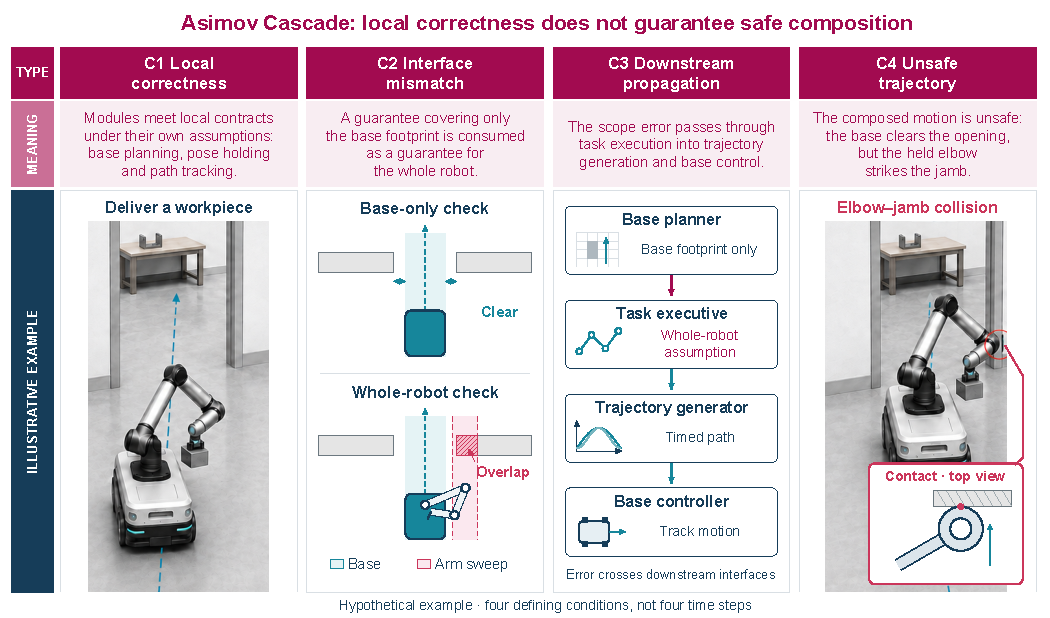
\includegraphics[width=0.72\textwidth,trim={0 13 0 17},clip]{fig01-doorway-hybrid-v4.pdf}
\caption{Hypothetical mobile-manipulator Asimov Cascade. In C1 each module meets its local specification. In C2 a base-only path guarantee is consumed as a whole-robot guarantee. In C3 the scope mismatch propagates through task execution, trajectory generation, and base control. In C4 the base clears the doorway, but the elbow-swept footprint intersects the jamb. The contact inset is a schematic top view, and the columns are defining conditions, not time steps. This is not a tested implementation or empirical evidence.}
\label{fig:concept}
\end{figure*}

\section{RELATED WORK}

\subsection{System-Level Robot Safety}

Interactions and unsafe control actions can dominate accident formation even when components pass local checks~\cite{leveson2011}. Full-stack safety, closed-loop anomaly detection, perception-failure recovery, and runtime-assurance architectures address this problem in deployed or simulated stacks~\cite{hsu2024,gupta2024,chakraborty2025,desai2019}, and name the mechanisms that our coding scheme seeks in patents. We apply this foundation at a different observation level, namely historical technology records.

\subsection{Patent-Based Technology forecasting}

Patent indicators support forecasting, but filing counts alone oversimplify lifecycle estimation~\cite{gao2013}. Multi-indicator HMM, diffusion, and natural-language approaches recover more of the technical content~\cite{lee2016,altuntas2015,arts2021}. Our count-based HMM and S-curve outputs are therefore exploratory descriptors rather than validated lifecycle states or forecasts. Recent work estimates performance-improvement rates from patent text~\cite{triulzi2020}, visualizes lifecycles with S-curve fits~\cite{ebisudani2025}, and identifies convergence with graph neural networks~\cite{zhu2022}. Closest to our corpus, topic modelling has been applied to humanoid-robot patents and publications to map the technology landscape~\cite{jang2016,kumari2019}. Those studies map topic structure, whereas we gate nominated mechanisms behind staged evidence review.

\subsection{Topic Models and Text-Based Inference}

BERTopic combines transformer embeddings, density clustering, and class-based TF-IDF~\cite{grootendorst2022}. PatentSBERTa supplies a patent-adapted embedding space~\cite{bekamiri2021}. STM relates topic prevalence to metadata~\cite{roberts2019}. Sample splitting reduces overfitting without making observational metadata causal~\cite{egami2022}. We therefore report held-out associations and avoid causal language. We combine embedding clustering (BERTopic), probabilistic prevalence (STM), and a semantic behavioral benchmark (ASIMOV). Agreement across unrelated model classes is harder to explain by shared artifacts.

\subsection{Benchmarks and Standards}

The ASIMOV Benchmark tests semantic action safety in foundation models, not physical subsystem interaction logs~\cite{sermanet2025}. The current editions are ISO 10218-1:2025 and ISO 10218-2:2025 (industrial robots) and ISO 13482:2014 (personal-care robots, under FDIS revision)~\cite{iso10218_1,iso10218_2,iso13482_2014,iso13482_fdis}. Two humanoid-specific efforts are closing this gap from the standards side, namely ISO/CD 25785-1, a committee draft on safety requirements for dynamically stable industrial mobile robots~\cite{iso25785_1}, and the IEEE Humanoid Study Group's 2025 pathway study for future humanoid standards~\cite{ieeehsg2025}. Standards can check nominated mechanisms against recognized hazards but cannot by themselves validate a patent-derived forecast.

\section{CONCEPTUAL MODEL}

\subsection{Formal Definition}

Let the robot stack be a directed graph $G = (V,E)$ of subsystems and interfaces. Subsystem $i$ satisfies a local contract $C_{i} = 1$ when its output meets its own specification under its assumed operating context, in the assume--guarantee sense of contract-based system design~\cite{benveniste2018}. For an interface $(i,j)$, $\mathrm{Compat}_{ij} = 1$ means that the output guaranteed by $i$ also satisfies the timing, frame, unit, mode, and priority assumptions of $j$.

For an ordered subsystem path $P$ containing at least two successive interfaces, the following conditions are necessary:

\begin{equation}
\begin{aligned}
\mathcal{AC}(P) = 1\ \Rightarrow \quad & C_{i} = 1\quad \forall i \in P, \\
 & \exists(i,j) \in P:\neg\mathrm{Compat}_{ij},\quad U(z_{T}) = 1.
\end{aligned}
\label{eq:cascade}
\end{equation}

where $z_{t}$ denotes the composed system state at time $t$, with $T$ the evaluation horizon, and $U(z_{T}) = 1$ marks an unsafe system trajectory. Equation~\eqref{eq:cascade} formalizes the locally checkable conditions C1, C2, and C4, while C3 is operationalized by requiring $P$ to contain at least two successive interfaces, so that the deviation must cross at least one downstream subsystem. We label the necessary conditions for later reference. (C1) every subsystem on the path satisfies its local contract. (C2) At least one interface on the path is incompatible. (C3) The incompatibility-induced state or context deviation propagates through at least one downstream subsystem. (C4) The system reaches an unsafe trajectory. C1, C2, and C4 alone characterize an unsafe compositional event but are not sufficient for a cascade. Without the propagation required by C3, a single incompatible interface is an interface failure, not an Asimov Cascade. Figure~\ref{fig:concept} instantiates this distinction on a hypothetical mobile manipulator passing a doorway. If the task planner discards the stale base-clearance estimate and re-plans from fresh state, the deviation dies at the interface (C1 and C2 hold, but C3 does not). In the depicted case, the base-only path guarantee is consumed as a whole-robot guarantee, the mismatch propagates through task execution, trajectory generation, and base control, and the elbow's swept footprint intersects the jamb, so C1 through C4 all hold. Actual injury is a separate event $H(z_{T}) = 1$ that additionally requires human exposure; a near miss may therefore satisfy $\mathcal{AC}(P) = 1$ while $H(z_{T}) = 0$.

We do not estimate $\mathcal{AC}(P)$, $C_{i}$, $\mathrm{Compat}_{ij}$, $U(z_{T})$, or $H(z_{T})$ from the patent corpus. The necessary-condition model specifies the runtime construct that motivates the coding scheme and bounds inference, since patents observe invention-level precursors of these conditions rather than the runtime events themselves, and establishing an actual cascade, unsafe trajectory, near miss, or injury requires runtime traces or physical tests. Patent publications are the unit of observation. An excerpt may nominate a safety barrier, a propagation node, or an interface mechanism (stale state, communication delay, mode mismatch), with $V$ guiding subsystem-role coding and $E$ and $P$ guiding interface and propagation-node coding. Topic~74, for instance, is a plausible propagation candidate whose patents establish neither an incompatible interface nor an unsafe trajectory.

\subsection{Observation Levels and Testable Hypothesis}

The formal event is a runtime property. The dataset contains invention disclosures, which can support the conclusion that a mechanism is a barrier or propagation node, but not that it participated in an accident. Our technology-level hypothesis is therefore conditional (H1). If innovation activity for a necessary safety barrier declines relative to the surrounding field without a substitute mechanism appearing, the system may become more exposed to interface-driven failures. H1 is falsified if declining barrier innovation is routinely offset by substitutes, or if standards and runtime records show no corresponding exposure. Patent observables test only the innovation-activity clauses, not the exposure consequence. The prioritization score operationalizes three patent-observable proxies for H1 (automated safety relevance, temporal decline, descriptive lifecycle position). It establishes neither mechanism necessity nor substitute absence, nor any cascade, unsafe trajectory, or injury, which require standards review and runtime or physical evidence.

Two score components deserve explicit non-claims. The decline probability $D_{j}$ is not a measure of safety deterioration but a review trigger on weakening innovation activity around an already safety-relevant mechanism. The lifecycle position $L_{j}$ is only a contextual weight for interpreting that decline, and late lifecycle may coincide with stabilization and standardization. Neither is interpreted as a safety measure in isolation. The score operationalizes a review-priority heuristic under H1, not a calibrated probability of failure, cascade occurrence, or injury.

\section{MATERIALS AND METHODS}

Figure~\ref{fig:pipeline} maps the discovery, prioritization, and validation logic that the remaining sections detail.

\begin{figure*}[!t]
\centering
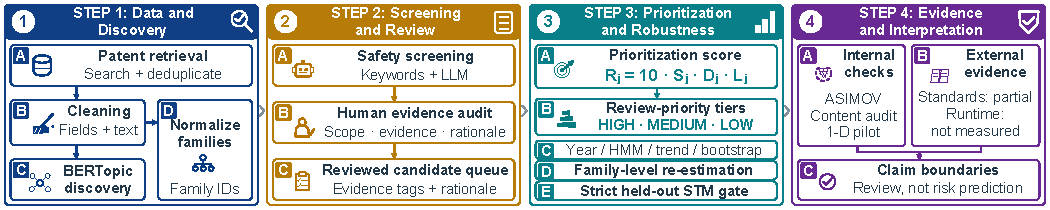
\includegraphics[width=0.85\textwidth]{fig02-original-style-v4.pdf}
\caption{Four-stage pipeline for discovery, screening/review, prioritization/robustness, and evidence interpretation. Family-normalized records feed Stage~3 checks. The held-out strict STM gate and author audit anchor nomination independently of the score. Tiers order review, not risk. ASIMOV, content audit, and 1-D pilot are internal/model-internal checks. Standards review is partial (6/18 pairs), and runtime evidence was not measured.}
\label{fig:pipeline}
\end{figure*}

\subsection{Corpus Construction}

The corpus was exported from incoPat~\cite{incopat} on July 18, 2026. The query searched titles and abstracts, requiring at least one term from a robot clause and at least one term from a safety clause. The robot clause comprised 5 terms targeting humanoid and legged embodied platforms(humanoid, ``bipedal robot,'' ``legged robot,'' ``embodied intelligence,'' and ``human robot'') and a safety clause of 20 terms (safety through adaptability). The verbatim Boolean string is archived in the reproducibility repository. For this study, the robot scope was defined as humanoid robots and closely related human--robot platforms in which direct interaction with humans is central to the operating context. Broader retrievals covering other robot categories, such as manufacturing manipulators, AGVs, and AMRs, were also tested but rejected as falling outside the scope. 

The cleaning pipeline removed non-analytic publication types, retained application years from 2006 onward, formed each document from the English abstract plus an English first claim when available, and required at least ten characters after concatenation (removing eleven empty records). The corpus contained 8,928 publication-level records (Figures~\ref{fig:corpus} and~\ref{fig:attrition}). Because 4,889 publications belonged to a multi-record simple family in the global index, we also ran a family-normalized primary re-estimation on 6,602 canonical simple families, each represented by its earliest-application record (159 representatives, 16 topic assignments, and 131 application years changed, and 6,703 raw identifiers collapsed to 6,602 after family-ID type normalization). BERTopic assignments and safety labels were held fixed, whereas yearly trends, five-state HMMs, logistic S-curves, prioritization scores, and a separate K=12 held-out STM were re-estimated from family representatives. Application year is the temporal index. Under an 18-month publication-lag rule applied to the July 2026 retrieval, both 2025 and 2026 are right-censored, except over fast-publishing, predominantly Chinese-authority routes, so the primary temporal analysis uses application years through 2024 (4,729 families), with 2025--2026 retained only as sensitivity cases (Table~\ref{tab:audit}).

\begin{figure}[!t]
\centering
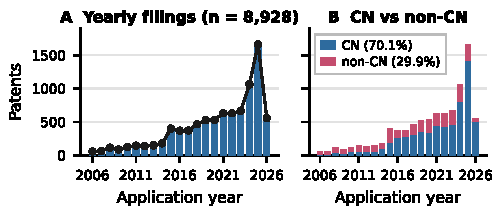
\includegraphics[width=0.74\columnwidth]{fig04_corpus.pdf}
\caption{Corpus overview of the 8,928 analyzed publications: (A) yearly filings and (B) authority split. Counts are publication-level. Under the 18-month publication-lag rule, 2025 and 2026 are both incomplete except over fast-publishing (mostly Chinese-authority) routes. The 70.1\% Chinese-authority share is treated as a limitation, not market-share evidence.}
\label{fig:corpus}
\end{figure}

\begin{figure}[!t]
\centering
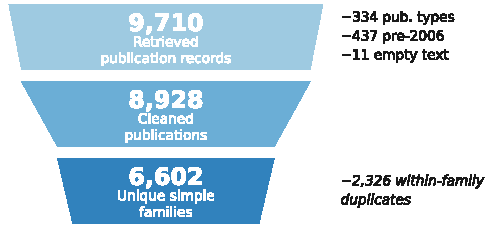
\includegraphics[width=0.70\columnwidth]{fig03_attrition.pdf}
\caption{Corpus attrition from retrieval to analysis: cleaning removed 782 records (334 non-analytic publication types, 437 pre-2006 applications, 11 empty texts). Family merging collapsed 8,928 publications into 6,602 simple families.}
\label{fig:attrition}
\end{figure}

\begin{figure}[!t]
\centering
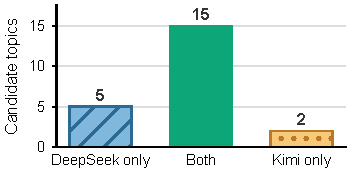
\includegraphics[width=0.72\columnwidth]{fig07_kimi.pdf}
\caption{DeepSeek--Kimi cross-model sensitivity: 76/77 valid, 90.8\% agreement ($\kappa = 0.750$), 15 shared candidates, and 7 disagreements. Kimi is not an independent reference label.}
\label{fig:kimi}
\end{figure}

\begin{table}[!t]
\centering
\caption{Corpus and model audit}
\label{tab:audit}
\footnotesize
\renewcommand{\arraystretch}{0.92}
\rowcolors{2}{gray!9}{white}
\begin{tabularx}{\columnwidth}{@{}>{\raggedright\arraybackslash}X >{\raggedright\arraybackslash}X >{\raggedright\arraybackslash}X@{}}
\toprule
\textbf{Quantity} & \textbf{Observed value} & \textbf{Verification (method, date)} \\
\midrule
Retrieved publication records & 9,710 & incoPat export log, 2026-07-18 \\
Analyzed publications / simple families & 8,928 / 6,602 & cleaning and family scripts, 2026-07-18 / 2026-08-29 \\
Application-year range & 2006-2026 (2025-2026 censored; primary $\le$2024) & number-export script, 2026-07-20 \\
Chinese publication-authority share & 70.1\% & number-export script, 2026-07-20 \\
BERTopic non-noise topics & 77 & frozen BERTopic output, 2026-07-20 \\
BERTopic noise documents & 2,698 (30.2\%) & frozen BERTopic output, 2026-07-20 \\
Automated safety candidates & 20 & frozen screening output, 2026-07-20 \\
STM train/test (publication; family) & 6,249/2,679; 4,621/1,981 & STM run outputs, 2026-08-08 \\
\bottomrule
\end{tabularx}
\end{table}

\subsection{BERTopic Discovery}

Documents were embedded with \texttt{AAUBS/PatentSBERTa\_V2}, reduced by cosine-UMAP (seed 42, \texttt{n\_neighbors}=15), and clustered by HDBSCAN (min\_cluster\_size=25)~\cite{grootendorst2022,bekamiri2021,mcinnes2017,mcinnes2018}. Labels used class-based TF-IDF, and noise documents were excluded from trend models. Four additional UMAP seeds yielded 75--83 topics, 31.7\%--34.3\% noise, and 14--16 of 20 candidates recovered at document-set Jaccard $\geq 0.5$. Parameter changes produced 43--152 topics with 10--12 candidates, and \texttt{all-MiniLM-L6-v2} recovered only 2, so claims are conditional on the reported granularity and embedding.

\subsection{Safety Screening and Evidence Review}

The prespecified screening procedure combined a keyword taxonomy with \texttt{deepseek-v4-flash} judgments over topic labels, keywords, and representative abstracts. DeepSeek-v4-flash was chosen for reliable structured JSON output at corpus scale, a practical choice rather than demonstrated superiority. Kimi, from an independent provider and training pipeline, was the cross-model sensitivity check, making agreement harder to attribute to shared model artifacts. The prompt returned a 0--5 score, category, confidence, and rationale; score $\geq 2$ formed the 20-topic review queue. Authors then reviewed patent excerpts and identifiers with each topic, assigning safety, harm-link, cascade-role, scope, and confidence labels. A topic was coded as direct safety only when its patents explicitly aimed to protect people or prevent human injury, as partial when explicit safety mechanisms were present but not the main contribution of most patents, as incidental when safety appeared only as a byproduct of another task, and as not-safety when safety terms were merely background wording. Harm-link labels distinguished injuries described in the patent text from injuries inferred across scenarios, and cascade-role labels followed the barrier and propagation-node definitions of Section III-A. Two authors independently labeled all 77 topics under this schema, disagreements were resolved by discussion with third-author arbitration, and the label definitions, both rating sheets, and the adjudication record are archived. To test dependence on a single stochastic draw, five independent re-screenings per model (DeepSeek and Kimi) were run over all 77 topics with the identical frozen prompt; the frozen historical output remains the primary record, reruns serving only as sensitivity analysis.

\subsection{Temporal Descriptors and Prioritization Score}

For each topic, yearly publication counts over the censored primary series (2006 through 2024) were segmented with a five-state Gaussian hidden Markov model, and a logistic S-curve was fitted to cumulative counts~\cite{rabiner1989}. The HMM supplied decline probability $D_{j}$, the S-curve supplied descriptive lifecycle weight $L_{j}$, and $S_{j} = s_{j}/5$ normalized the automated safety-relevance score. The candidate-prioritization score is $R_{j} = 10S_{j}D_{j}L_{j}$.

In words, $R_{j}$ scales the review priority of a safety-relevant topic whose innovation activity is declining, with lifecycle position weighting how that decline should be read. It does not scale danger. Candidates were assigned to review-priority tiers (HIGH when $R_{j} \geq 0.08$, MEDIUM when $0.02 \leq R_{j} < 0.08$, and LOW otherwise, conditional on $s_{j} \geq 2$), where HIGH denotes review priority rather than validated safety risk. These cutoffs are heuristic review-queue thresholds, not learned probabilities or calibrated risk boundaries. Under the censored-2024 primary, the HIGH tier contains three candidates with $R_{j} \in [0.35, 5.60]$. The lowest HIGH score is $4.4\times$ the HIGH cutoff and $5.8\times$ the highest non-HIGH candidate score (0.06), so the cutoff separates a gap in the score distribution rather than splitting a cluster. We tested sensitivity to deleting or annualizing right-censored years, truncating the primary series at 2024, two to five HMM states, simpler trend baselines, and 500 document-level bootstrap replicates.

\subsection{Structural Topic Model and Cross-Model Gate}

STM used $K = 12$ topics and a fixed 70/30 split with seed 12345~\cite{roberts2019,egami2022}. $K = 12$ was selected on the same split by held-out likelihood. The training model included a smooth application-year term, ten standardized time-related patent covariates, IPC section, publication authority, and authority-dependent content. Test documents were projected into the fixed topic space and held-out topic proportions regressed on the same terms, producing 120 topic--covariate tests. We report both nominal $p < 0.05$ counts and Benjamini--Hochberg false-discovery-rate control at $q \leq 0.05$~\cite{benjamini1995}.

For the cross-model gate, documents in each BERTopic cluster were mapped to their dominant held-out STM topic. The provisional rule labeled a candidate as passing the gate when that STM topic had a negative nominal ($p < 0.05$ before correction) association for disclosure speed or priority urgency. The negative direction was prespecified before examining the held-out fits, as declining speed or urgency is the direction implied by H1. This stress-tests model convergence, not causal validity. A strict candidate must also pass human scope review and the multiple-testing gate.

\subsection{ASIMOV Falsification Test and Role Diagnostic}

The ASIMOV analysis was treated as a falsification-oriented internal stress test, not external validation. Patent documents and 319 ASIMOV scenarios were embedded in the same frozen PatentSBERTa space, and each scenario received a similarity-weighted exposure to nearby patent topics via k-nearest neighbors in cosine distance (k=50 primary, with k=25 and 100 as sensitivities, 1,276 scenario-question observations, and 308 scenarios in the three-seed Kimi intersection). Cluster-robust logistic regressions related frozen DeepSeek and three-seed Kimi-majority errors to exposure, controlling for subquestion and log scenario length, complemented by a topic-level Spearman test.

A post hoc construct diagnostic decomposed exposure by the author-audited topic roles (12 safety barriers, 5 propagation nodes, 3 other topics), estimated jointly for the 2,395-publication and 1,773 earliest-family-representative pools with Benjamini--Hochberg correction and leave-one-role-topic-out checks (settings archived in the reproducibility repository).

\subsection{Blinded Structured Content Audit of Topics 22 and 25}
To characterize what the two strict-gate clusters disclose, a blinded structured single-reviewer content audit coded their canonical families (49 for Topic 22 and 38 for Topic 25, Section IV-A) using a frozen codebook over each family's representative text (first claim, then abstract, then title), recording direct safety relevance, contact-safety context, force or proximity sensing, sensor--decision--response chain completeness, explicit humanoid scope, cross-subsystem propagation language, and off-topic status, with an evidence quote and confidence per record. Records coded Unclear leave each indicator's denominator by that indicator's rule. The reviewer was blinded to topic identity and model outputs until coding was complete. Contrasts used two-sided Fisher exact tests with Benjamini--Hochberg correction, robust under a duplicate-text collapse sensitivity analysis (79 rows, 42 versus 37). Eighteen twice-coded records give same-session repeat agreement. The audit covers the middle two of four evidence levels (model-generated cluster, author interpretation, statistical comparison, external validation).

\subsection{Controlled Propagation Simulation Pilot}
As a model-internal mechanistic probe of the propagation condition C3 (Section III-A), we preregistered a one-dimensional state-space controlled simulation of an approach-and-stop interaction (a one-dimensional projection of the doorway scenario in Figure~\ref{fig:concept}) guarded by a safety-margin monitor. Five conditions (labels \textsc{Base}--\textsc{Rescue} distinct from C1--C4) were defined. \textsc{Base} is a frozen baseline, \textsc{Delay} injects a 25--200 ms timestamp delay into the monitor's state estimate, \textsc{Thresh} applies a one-sided $\pm 0.03$/$\pm 0.06$ m offset on a shared safety threshold, \textsc{Bias} applies a transient $+0.08$ m position-sensor bias (an ordinary component failure), and \textsc{Rescue} is a matched conservative rescue pairing a 25 ms timestamp-age gate with a shared-threshold contract check. The design comprised 66 cells with 50 frozen seeds each (3,300 formal trials) under common random numbers, frozen before any simulation run.

A trial is PROPAGATED only if the interface mismatch acts first, the safety margin is breached afterward (gap below $d_{\mathrm{safe}}=0.2$ m for a prespecified sustained duration, with an approach-speed rule at crossing), and every modeled local contract remains satisfied. Earlier breaches are recorded as BREACH\_UNORDERED, never as propagation. Each \textsc{Delay} or \textsc{Thresh} cell was tested against its common-random-number \textsc{Base} cell (exact McNemar test, Benjamini--Hochberg correction, paired risk differences, seed-level bootstrap confidence intervals).

One deviation was registered. Trial duration was extended from 4.0 s to 8.0 s under a preregistered calibration rule (reason and re-hash logged in the simulation audit report).

\section{RESULTS}

\subsection{Topic Landscape and Human Evidence Audit}

Seventy-seven non-noise topics emerged from the 8,928-publication corpus, alongside 2,698 noise documents (30.2\%); the frozen screen nominated 20 of the 77 topics, leaving 57 below threshold. Table~\ref{tab:review} and Figure~\ref{fig:audit} summarize the review of the 20 screened candidates. The adjudicated safety labels assign 3 direct, 4 partial, 8 incidental, and 5 not-safety, while the 12 barrier and 5 propagation-node roles come from the first-pass audit. A frozen Kimi run returned 76/77 valid outputs and agreed with DeepSeek on 69/76 labels (90.8\%, $\kappa = 0.750$, 15 shared candidates, Figure~\ref{fig:kimi}). The seven disagreements (Topics 0, 1, 25, 28, 34, 64, and 74) remain audit cases, and missing Topic~69 was not selectively rerun. Two authors then independently adjudicated all 77 topics under the same schema. Agreement was 70.1\% on the five-way safety judgment ($\kappa = 0.467$), 68.8\% on the harm link ($\kappa = 0.371$), 45.5\% on the cascade role ($\kappa = 0.244$), and 89.6\% on the binary candidate decision ($\kappa = 0.606$). The 23 five-way disagreements were resolved by discussion with third-author arbitration. Against the adjudicated full-corpus labels, the screen reached recall 7/13 and precision 7/20 (Table~\ref{tab:layers}), so it is a coarse triage filter and mechanism nomination rests on the strict gates rather than on screening precision.



\begin{table}[!t]
\centering
\caption{Human review of 20 screened candidates (safety-judgment rows report the adjudicated labels; harm-link and cascade-role rows retain the first-pass audit)}
\label{tab:review}
\footnotesize
\renewcommand{\arraystretch}{0.92}
\rowcolors{2}{gray!9}{white}
\begin{tabularx}{\columnwidth}{@{}>{\raggedright\arraybackslash}X >{\raggedright\arraybackslash}X r@{}}
\toprule
\textbf{Field} & \textbf{Decision} & $\mathbf{n}$ \\
\midrule
Safety judgment & Direct & 3 \\
& Partial & 4 \\
& Incidental & 8 \\
& Not safety & 5 \\
\addlinespace
Human-harm link & Direct & 4 \\
& Indirect & 15 \\
& Unclear & 1 \\
\addlinespace
Cascade role & Safety barrier & 12 \\
& Propagation node & 5 \\
& Context only & 1 \\
& Out of scope & 1 \\
& Unclear & 1 \\
\bottomrule
\end{tabularx}
\end{table}

\begin{figure*}[!t]
\centering
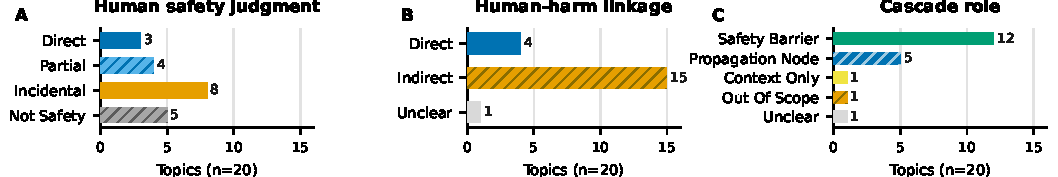
\includegraphics[width=0.66\textwidth]{fig05_audit.pdf}
\caption{Human evidence audit: review decisions for the 20 screened candidates. (A) Human safety judgment (adjudicated labels). (B) Human-harm linkage and (C) cascade role (first-pass audit); counts per Table~\ref{tab:review}, dual-author adjudication statistics in Section V-A.}
\label{fig:audit}
\end{figure*}



Across five re-screenings per model, DeepSeek's queue was stable (mean pairwise Jaccard 0.956, 17 of the 20 frozen candidates reproduced in at least four of five runs, and no new topic ever nominated). Paired cross-model runs agreed on 90.6\% of binary labels (mean $\kappa = 0.715$), consistent with the frozen single-run comparison, and neither model is a reference label.

\subsection{Family Normalization and Right-Censoring Reshape the HIGH Set}

The score produced 5 HIGH, 4 MEDIUM, and 11 LOW candidates (Figure~\ref{fig:gates}). Under the adjudicated labels, the HIGH set comprises two direct-safety topics (22 and 25), one partial-safety topic (40), and two topics adjudicated Not-Safety (7 and 29). Topics 25 and 40 are cross-platform comparators, and Topic~22 has the clearest force evidence. Read against the review's own scope notes, only Topic~7 (vehicle lane-changing and human-like driving patents) was judged out of scope. Topic~29 (display, reception, and service robots whose safety devices are incidental to the inventions) would also fall outside under a humanoid-strict reading (Table~\ref{tab:layers}). Two further raw-HIGH topics, 22 and 25, center on generic collaborative and industrial robots rather than humanoid platforms, a breadth traceable to the retrieval query (Section IV-A). We therefore report scope status per topic for the frozen corpus.

\begin{figure}[!t]
\centering
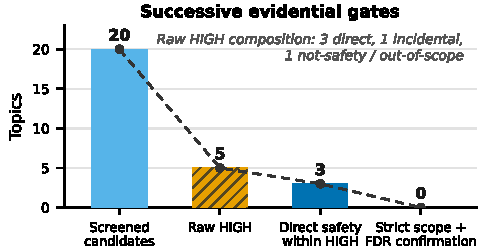
\includegraphics[width=0.85\columnwidth]{fig06_gates.pdf}
\caption{Successive evidential gates. The frozen screen nominated 20 candidates from 77 topics; five ranked publication-level HIGH. The censored-2024 family primary contracts the HIGH tier to Topics 7, 25, and 40, and the held-out strict family-level gate is passed by Topics 22 and 25. Tiers order review, not risk.}
\label{fig:gates}
\end{figure}

Topic~22 clusters force-aware human--robot interaction safety patents that detect and limit external force in contact, spanning generic collaboration rather than one humanoid platform. The audit assigned Direct safety, Direct harm link, and barrier role at High confidence (Table~\ref{tab:review}). These barriers sit where locally valid commands meet a changed contact context (C2). Whether force-limiting barriers engage correctly under mid-execution context shifts is bench-testable.

Under the censored-2024 family primary, the HIGH set contracts from the publication-level five (Topics 7, 22, 25, 29, and 40) to Topics 7, 25, and 40. Topic 22 moves to MEDIUM. Its full-series decline probability of 0.80 collapses to 0.01 once the incompletely published 2025--2026 edge is removed. Its former HIGH label was edge-driven, not a durable decline. Only Topic 25 retains the HIGH tier under every recent-year perturbation (deleting, annualizing, or truncating the censored years). Topic 7 flips under two of three variants, and Topic 40 enters HIGH only under the truncated primary.

Across the 20 candidates, six review-priority tier assignments change between the full and the censored-2024 family series, and score ranks correlate moderately (Spearman $\rho = 0.487$, p = .030). Across all 77 topics, the HMM trend direction changes for 51 and the S-curve lifecycle stage for 26. Topic 7 remains HIGH in the primary but was independently judged out of scope (Table~\ref{tab:layers} and Figure~\ref{fig:ranks}), and only Topic 25 kept a robust bootstrap HIGH probability (Table~\ref{tab:layers}).

Because the decline score is this edge-sensitive, mechanism nomination rests on the strict gate (Section V-C) and the human audit, with Topic 22 carrying the strongest audit evidence (Section V-E).

\begin{figure}[!t]
\centering
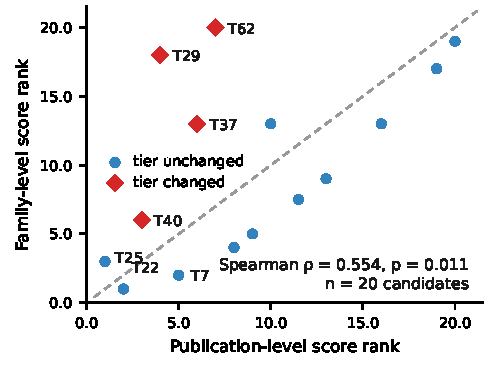
\includegraphics[width=0.55\columnwidth]{fig08_ranks.pdf}
\caption{Publication-level versus family-level (full-series) score ranks for the 20 screened candidates (Spearman $\rho = 0.554$, p = .011). Diamonds mark the four candidates whose review-priority tier changed in the publication-level-to-family-level comparison (e.g., Topic 29 HIGH to LOW and Topic 40 HIGH to MEDIUM); the separate full-series-to-censored-2024 comparison is reported in the text ($\rho = 0.487$).}
\label{fig:ranks}
\end{figure}

\subsection{Publication- and Family-Level STM Gates}

In the publication-level STM, 38 of 120 held-out tests were nominal and 19 survived Benjamini--Hochberg correction. Topic 7 was the only nominal cross-model candidate (p = .0488) but was author-reviewed as Not-Safety/out-of-scope and failed multiplicity (q = .1542). No reviewed in-scope HIGH candidate passed both gates (Table~\ref{tab:layers}). The independently refitted family STM yielded 29 nominal and 18 BH-retained effects. Topics 22 and 25 both mapped to the same dominant STM topic with a negative disclosure-speed association ($\beta=-0.0365$, p = $7.67\times10^{-6}$, q = $1.15\times10^{-4}$) and passed the strict gate. These two gate-passing results share one STM topic, so they are one strand of evidence, not two independent replications. Repeated family members inflate publication-level prevalence for their topic, so one earliest representative per family shifts topic projection (demoting Topic 7, promoting Topic 22). These results nominate both topics for standards and runtime testing.

\subsection{Frozen ASIMOV Reproduction and Construct Diagnostic}

The frozen publication-level pooled models exactly reproduced the reported inverse coefficients. At k=50, DeepSeek gave $\beta=-3.818$ (p = .0007) and Kimi majority voting $\beta=-2.263$ (p = .1005). The k=25 and k=100 sensitivities were likewise negative for both models. Reproduction meant agreement within $10^{-10}$ for exposures and $10^{-9}$ for coefficients. The topic-level association remained null ($\rho = -.231$, permutation p = .3669).

In the post hoc k=50 role model, DeepSeek barrier exposure was inversely associated with error in the publication pool ($\beta=-.317$ per SD, 95\% CI $[-.482,-.153]$, q = .0009) and family pool ($\beta=-.215$, 95\% CI $[-.381,-.050]$, q = .0216). Propagation exposure was null (publication $\beta=.104$, q = .425; family $\beta=-.030$, q = .730), and no Kimi role term survived BH correction (minimum $q = 0.13$ across both pools and three k values). DeepSeek barrier signs remained negative across k=25,50,100 in both pools, but omitting Topic 22 reversed the family barrier sign (Table~\ref{tab:loto}), and propagation estimates were unstable (Figure~\ref{fig:stress}). \textbf{The ASIMOV result does not validate the candidate-prioritization score.} The implication is a scope boundary, not a refutation. The score's claims rest on the strict held-out gate and the human audit, while this test can only bound, not establish, the technology-to-safety link. The inverse association was concentrated in the DeepSeek safety-barrier term, with propagation and Kimi role terms null.

\begin{table}[!t]
\centering
\caption{Leave-one-topic-out diagnostic for the barrier association}
\label{tab:loto}
\footnotesize
\renewcommand{\arraystretch}{0.92}
\rowcolors{2}{gray!9}{white}
\begin{tabularx}{\columnwidth}{@{}l >{\raggedright\arraybackslash}X >{\raggedright\arraybackslash}X@{}}
\toprule
\textbf{Model and pool} & \textbf{Full model} & \textbf{Omitting Topic 22} \\
\midrule
DeepSeek, family & $-0.215$ (p = .011) & $+0.208$ (p = .114), sign reversed \\
KimiMV, family & $-0.079$ (p = .442) & $+0.383$ (p = .031), sign reversed \\
DeepSeek, publication & $-0.317$ (q = .0009) & $-0.372$ (p = .001), robust \\
KimiMV, publication & not retained ($q \geq .291$) & $-0.208$ (p = .050), robust \\
\bottomrule
\end{tabularx}
\end{table}

\begin{figure*}[!t]
\centering
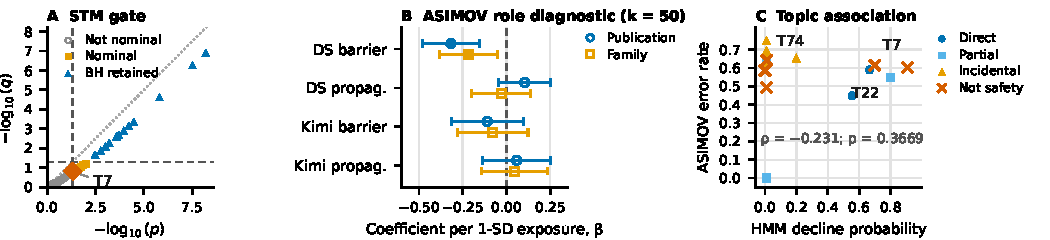
\includegraphics[width=0.66\textwidth]{fig09_stress.pdf}
\caption{Internal stress tests and construct diagnosis. (A) Publication-STM held-out tests (Section V-C); the diamond marks Topic 7. (B) Post hoc k=50 role coefficients with cluster-robust 95\% CIs; filled symbols denote BH $q\leq.05$; DeepSeek barrier terms are negative in both pools. (C) The publication-level topic association is null (Spearman $\rho = -.231$, p = .3669). Internal stress tests, not external validation or injury forecasting.}
\label{fig:stress}
\end{figure*}


\subsection{Content Audit Findings for Topics 22 and 25}
The audit found Topic 22 to be a model-generated patent cluster enriched for force-aware human--robot interaction safety mechanisms. Direct safety relevance was coded in 34 of 49 Topic 22 families (69.4\%) versus 14 of 38 Topic 25 families (36.8\%, exploratory Fisher contrast, BH q = .00774); force or proximity sensing in 38 of 48 versus 19 of 37 (79.2\% versus 51.4\%, q = .0142), and a complete sensor--decision--response chain in 32 of 49 versus 6 of 36 (65.3\% versus 16.7\%, q = $5.72\times10^{-5}$). Off-topic coding was less frequent in Topic 22 (5 of 49, 10.2\%) than in Topic 25 (19 of 38, 50.0\%, q = .000229). No family in either cluster explicitly claimed a humanoid-specific scope (0 of 49 and 0 of 38), and explicit cross-subsystem propagation language was rare and not significantly different between clusters (2 of 49 versus 0 of 38, q = .586). All contrasts kept their direction and significance under the duplicate-text collapse sensitivity analysis, and the 18 twice-coded records agreed 100\% on every categorical field (same-session repeat agreement, Section IV-G). The audit therefore supports a mechanism-enrichment reading of Topic 22, not a humanoid-specific, collision-verified, or real-world cascade category.

\subsection{Simulation Pilot: Ordered Margin Erosion with Satisfied Local Contracts}
All 3,300 preregistered trials completed (Figure~\ref{fig:sim}). Under \textsc{Base}, 150 of 150 trials remained contained with all local contracts satisfied. Under \textsc{Delay}, 369 of 900 trials propagated (41.0\%, Wilson 95\% CI 37.8--44.2\%) and 244 further trials breached the margin before the delayed trigger (BREACH\_UNORDERED, not propagation). Under \textsc{Thresh}, 149 of 600 trials propagated (24.8\%, 95\% CI 21.5--28.4\%) with 151 unordered breaches.

All 518 propagated trials passed every modeled local contract and satisfied the frozen strict event order. The delay response was non-monotone. Propagation concentrated at intermediate delays, and the largest delays produced unordered breaches, so a larger delay does not imply stronger propagation. Propagation occurs only while the delayed trigger precedes the margin breach, and slower approaches breach later, shifting this window to longer delays. The 0.15 m/s band therefore sits at 150 ms (Figure~\ref{fig:sim}). All 150 \textsc{Bias} trials were ordinary component failures. The injected bias violates the local contract, so the cascade precondition cannot hold.

\textsc{Rescue} eliminated propagation in every paired cell that had propagated under its parent condition (0 of 1,500 propagated, no margin breach, Wilson upper bound 0.26\%). This is a model-specific conservative rescue, not a general safety prescription. The synthetic contact force was 0 N in all 3,300 trials, precluding any injury interpretation. The frozen outcome classification was PILOT\_SUPPORT.

\begin{figure}[!t]
\centering
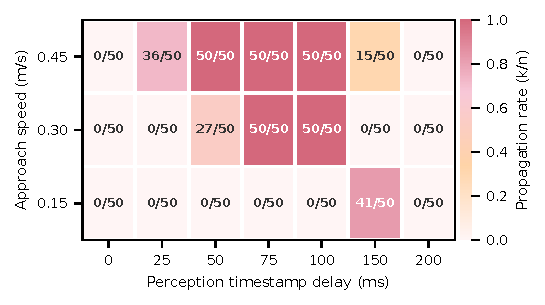
\includegraphics[width=0.85\columnwidth]{fig11_sim_heatmap.pdf}
\caption{Controlled one-dimensional simulation pilot under the timestamp-delay condition \textsc{Delay} (50 frozen seeds per cell; delay 0 ms is the matched \textsc{Base} baseline). A cell counts a trial only when the frozen strict event order held with all modeled local contracts passing (PROPAGATED); earlier breaches are BREACH\_UNORDERED, not propagation. Simulation results only; not evidence about real robots.}
\label{fig:sim}
\end{figure}

\section{DISCUSSION}

\subsection{What the Present Evidence Establishes}

The present evidence supports an auditable evidence architecture rather than accident prediction. Patent excerpts nominate barriers and propagation mechanisms at subsystem interfaces (RQ1), and the blinded content audit supports Topic 22's enrichment for force-aware human--robot interaction safety mechanisms (RQ3). Family normalization and right-censoring materially change score ranks and tiers, with only Topic 25 HIGH across all variants (RQ2). The family STM result for Topics 22 and 25 is a focused hypothesis for standards and runtime testing, establishing neither frequency, failure, nor injury consequence (RQ3). The discordant publication- and family-level gates and the ASIMOV stress test delimit internal checks from external validation (RQ4), and the controlled 1-D pilot supplies model-internal support for ordered safety-margin erosion under bounded interface mismatch (RQ5).

\subsection{Validation Layers and Open Gaps}

\begin{figure*}[!t]
\centering
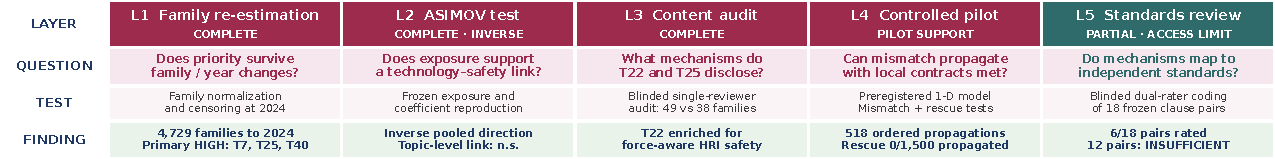
\includegraphics[width=0.88\textwidth]{fig10_layers_tablestyle.pdf}
\caption{Evidence layers and their status. L1 (family re-estimation, censored-2024 primary) and L2 (ASIMOV test) are complete, L2 returning an inverse result. L3 (content audit of Topics 22/25) and L4 (1-D simulation pilot) are author-side and model-internal checks, while L5 (independent standards review) is partial under full-text access limits (6 of 18 pairs rated).}
\label{fig:layers}
\end{figure*}

Table~\ref{tab:layers} and Figure~\ref{fig:layers} separate completed corpus, pipeline, and label checks from evidence absent for the technology-to-safety link. Patent topic discovery, content audit, and 1-D mechanistic simulation observe different constructs (disclosed mechanisms, coded content, and model-internal dynamics), and runtime evidence was not observed.

\begin{table*}[!b]
\centering
\caption{Successive evidential gates and validation layers}
\label{tab:layers}
\scriptsize
\renewcommand{\arraystretch}{0.92}
\rowcolors{2}{gray!9}{white}
\begin{tabularx}{\textwidth}{@{}>{\raggedright\arraybackslash}X >{\raggedright\arraybackslash}X >{\raggedright\arraybackslash}X@{}}
\toprule
\textbf{Gate or test} & \textbf{Result} & \textbf{What would change this} \\
\midrule
Automated safety candidates & 20 & Full-corpus adjudication complete (77-topic dual review, $\kappa$ = 0.467/0.606) \\
Out-of-scope among raw HIGH & 1 (2 under a humanoid-strict reading) & A humanoid/legged must-have term or CPC anchor in the query \\
STM held-out tests, nominal / BH-retained (publication; family) & 38/19 of 120; 29/18 of 120 & A different covariate set, split, or multiplicity rule \\
Cross-model and strict-gate outcomes (publication; family) & Topic 7; Topics 22 and 25 / 0; 2 (Topics 22 and 25) & A different topic granularity; independent family-level replication \\
ASIMOV scenario coefficient and role split, k = 50 & DeepSeek $-3.818$ (p = .0007), Kimi MV $-2.263$ (p = .1005); barrier $-.317$ (q = .0009) / $-.215$ (q = .0216), propagation/Kimi null & A positive, concordant replication across labelers, k, and roles \\
Score robustness: bootstrap P(HIGH), Topic 25 vs. others & 0.94 vs. 0.24-0.48 & Longer, uncensored annual series \\
Kimi-DeepSeek agreement and multi-run stability & 69/76 (90.8\%), $\kappa = 0.750$; DeepSeek Jaccard 0.956, 17/20 stable; cross-model 90.6\%, $\kappa = 0.715$ & Independent adjudication by an outside team \\
Family-normalized re-estimation (censored-2024 primary) & 6,602 families (4,729 $\le$2024); HIGH $5\rightarrow3$ (Topics 7, 25, 40); tier assignments changed 6/20 & Retraining on all family members; longer uncensored series \\
Fused queue, within-queue PPV & 7/20 (35\%); full-corpus recall 7/13, precision 7/20, specificity 51/64, F1 0.42 & Replication of the screen on an independent corpus \\
Structured content audit (Topics 22/25) & 49/38 canonical families coded; Topic 22 enriched for force-aware interaction safety; explicit propagation 2/49, not significant & An independent second-reviewer audit \\
Controlled 1-D simulation pilot & PILOT\_SUPPORT; 518 ordered propagations under mismatch; rescue 0/1,500; contact force 0 N & Real-robot and richer world-model validation \\
Standards dual-rater review (frozen 18 pairs) & 6/18 complete (access-limited); agreement 6/6; 5 applicable consensus PARTIAL; 0 decoy false mappings; 12 INSUFFICIENT & Full normative-text access and a larger complete set \\
\bottomrule
\end{tabularx}
\end{table*}

\subsection{External Standards-Mapping Design}

Safety standards encode recognized hazards, safeguards, interface requirements, and verification duties independently of our ranking model, and so serve as a construct-and-coverage reference, not a certification claim. We froze an 18-pair evaluation design for the two reviewed direct-safety mechanisms passing the family-level strict gate (Topics 22 and 25), covering ISO 10218-1:2025, ISO 10218-2:2025, and ISO 13482:2014 with two prespecified applicable clauses and one within-standard negative-control decoy per mechanism--standard combination (12 applicable pairs, 6 decoys)~\cite{iso10218_1,iso10218_2,iso13482_2014}. Two reviewers, blinded to the applicable/decoy key, independently coded DIRECT, PARTIAL, NONE, or INSUFFICIENT. With authorized access to the two ISO 10218 parts, 6 of the 18 pairs were fully coded (5 applicable, 1 decoy). The reviewers agreed on all 6, mapped 5 of 5 accessible applicable pairs as PARTIAL, and correctly rejected the decoy (0\% false mapping). The remaining 12 pairs were coded INSUFFICIENT by at least one reviewer at the cutoff, so standards-based construct coverage remains partial and no kappa is reported at this sample size.

\subsection{Limitations}

Generalization is limited by the 70.1\% Chinese-authority share, search scope, and BERTopic settings. Publication lag leaves 2025--2026 incomplete at the July 2026 retrieval, motivating the primary analysis through 2024 (Section IV-A). Family normalization depends on simple-family identifiers and a single earliest representative, and the publication and family analyses disagree on HIGH membership and strict STM confirmation, so neither is a calibrated risk model. Disclosure is not implementation either. Many patented mechanisms are never built or fielded, and the corpus cannot separate deployed safeguards from unbuilt proposals, so nominated mechanisms need the standards-mapping and runtime checks of Section VI-C before any engineering conclusion.

All 77 topics received independent dual-author adjudication, but the label task is intrinsically subjective (Section V-A), and the full-corpus screen is a coarse triage filter rather than a precise classifier. The role-separated ASIMOV analysis was post hoc, reused author-assigned roles, and had strongly unequal neighbor mass (barrier 88.2\% versus propagation 11.6\%, with the residual 0.3\% lying outside these two roles). Its family barrier estimate also depended on Topic 22. LLM robustness was assessed with only two models and one frozen prompt. Differing temperatures confound cross-model comparisons. Short annual series, filing-based S-curves, heuristic thresholds, fixed STM K=12, and cross-domain ASIMOV errors further limit inference~\cite{gao2013,lee2016}.

The standards ratings cover 6 of the 18 frozen pairs, and no runtime or near-miss traces were included. Such evidence would still not convert the prioritization score into an injury predictor.

Manual content coding limits scalability and remains subjective. The single-reviewer audit measures repeat agreement, not inter-rater reliability. Future work should evaluate LLM-assisted coding against independent human ratings. Topic 22 is neither humanoid-specific nor propagation-explicit (Section V-E), so the audit supports mechanism enrichment rather than a verified collision-protection or cascade category.

The simulation is a model-internal probe only. Its non-monotone delay response forbids reading greater delay as greater propagation, the \textsc{Rescue} result is a matched conservative rescue within this construct rather than a general fix, and the 0 N synthetic contact force precludes any injury interpretation (Section V-F). Scaling up proceeds in stages, from multi-dimensional state spaces with contact dynamics in a physics simulator, through richer mismatch families (frame, unit, mode, priority), to instrumented bench tests on a mobile manipulator, each stage trading part of the pilot's strict event-order control for ecological realism.

\section{CONCLUSION}

This paper defined the Asimov Cascade and proposed an evidence-gated technology-management method for patent monitoring when subsystem-level incident data are not public. Under the censored-2024 family primary, the HIGH set contracts from five publication-level topics to Topics 7, 25, and 40, and only Topic 25 keeps its tier under every recent-year perturbation. Mechanism nomination rests on the strict held-out STM gate, which finds Topics 22 and 25 passing its prespecified criterion, and on the human audit. The frozen ASIMOV result reproduced exactly, retaining the inverse, barrier-concentrated direction. The blinded content audit identifies Topic 22's enrichment for force-aware human--robot interaction safety mechanisms, and the preregistered one-dimensional pilot demonstrates ordered safety-margin erosion with modeled local contracts satisfied. Together, these results support mechanism monitoring and model-internal plausibility, not real-world cascade or injury prediction. Generalization beyond patents requires completed standards mappings (6 of 18 pairs coded), runtime or near-miss traces, and richer world models.

\section*{ACKNOWLEDGMENT}

[Funding statement anonymized for double-anonymous review.]

Automated topic-screening judgments were generated by DeepSeek through a rolling model alias at temperature 0.1 (Section~IV-C). Kimi served only for cross-model sensitivity. OpenAI Codex assisted language editing, code review, and vector-layout drafting for Figures~\ref{fig:concept} and~\ref{fig:pipeline}. The standards-clause coding notes in Section~VI-C were drafted by the reviewers with assistance from AI tools. The authors reviewed all judgments, code, numbers, text, and figures and remain responsible for the analysis. All prompts, settings, seeds, and records are archived in the reproducibility repository. \textit{A note on the name.} ``Asimov Cascade'' is a homage to Isaac Asimov's fictional laws of robotics. The phrase also names a decoy catastrophe in \textit{Rick and Morty} (Season 5, ``Mortyplicity''). Our construct is neither story. It is a system-level framework in which locally correct subsystems compose into an unsafe outcome, and no one is to blame. We chose the name with affection, and we take the framework itself seriously.

\scriptsize\linespread{0.62}\selectfont
\setlength{\itemsep}{-2.2pt}\setlength{\parsep}{0pt}
\begin{thebibliography}{37}

\bibitem{asimov1950}
I.~Asimov, \textit{I, Robot}. New York, NY, USA: Gnome Press, 1950.

\bibitem{leveson2011}
N.~G. Leveson, \textit{Engineering a Safer World: Systems Thinking Applied to Safety}. Cambridge, MA, USA: MIT Press, 2011.

\bibitem{hsu2024}
K.-C. Hsu, ``Scaling full-stack safety for learning-enabled robot autonomy,'' Ph.D. dissertation, Dept. Elect. Comput. Eng., Princeton Univ., Princeton, NJ, USA, 2024.

\bibitem{gupta2024}
A.~Gupta, K.~Chakraborty, and S.~Bansal, ``Detecting and mitigating system-level anomalies of vision-based controllers,'' in \textit{Proc. IEEE Int. Conf. Robotics and Automation (ICRA)}, 2024, pp.~6844--6850.

\bibitem{chakraborty2025}
K.~Chakraborty, Z.~Feng, S.~Veer, A.~Sharma, B.~Ivanovic, M.~Pavone, and S.~Bansal, ``System-level safety monitoring and recovery for perception failures in autonomous vehicles,'' in \textit{Proc. IEEE Int. Conf. Robotics and Automation (ICRA)}, 2025; arXiv:2409.17630.

\bibitem{desai2019}
A.~Desai, S.~Ghosh, S.~A. Seshia, N.~Shankar, and A.~Tiwari, ``SOTER: A runtime assurance framework for programming safe robotics systems,'' in \textit{Proc. 49th IEEE/IFIP Int. Conf. Dependable Systems and Networks (DSN)}, 2019.

\bibitem{gao2013}
L.~Gao, A.~L. Porter, J.~Wang, S.~Fang, X.~Zhang, T.~Ma, W.~Wang, and L.~Huang, ``Technology life cycle analysis method based on patent documents,'' \textit{Technological Forecasting and Social Change}, vol.~80, no.~3, pp.~398--407, 2013.

\bibitem{lee2016}
C.~Lee, J.~Kim, O.~Kwon, and H.-G. Woo, ``Stochastic technology life cycle analysis using multiple patent indicators,'' \textit{Technological Forecasting and Social Change}, vol.~106, pp.~53--64, 2016.

\bibitem{altuntas2015}
S.~Altuntas, T.~Dereli, and A.~Kusiak, ``Forecasting technology success based on patent data,'' \textit{Technological Forecasting and Social Change}, vol.~96, pp.~202--214, 2015.

\bibitem{arts2021}
S.~Arts, J.~Hou, and J.~C. Gomez, ``Natural language processing to identify the creation and impact of new technologies in patent text: Code, data, and new measures,'' \textit{Research Policy}, vol.~50, no.~2, Art.~no.~104144, 2021.

\bibitem{grootendorst2022}
M.~Grootendorst, ``BERTopic: Neural topic modeling with a class-based TF-IDF procedure,'' arXiv:2203.05794, 2022.

\bibitem{bekamiri2021}
H.~Bekamiri, D.~Hain, and R.~Jurowetzki, ``PatentSBERTa: A deep NLP based hybrid model for patent distance and classification using augmented SBERT,'' arXiv:2103.11933, 2021.

\bibitem{mcinnes2017}
L.~McInnes, J.~Healy, and S.~Astels, ``hdbscan: Hierarchical density based clustering,'' \textit{Journal of Open Source Software}, vol.~2, no.~11, Art.~no.~205, 2017.

\bibitem{mcinnes2018}
L.~McInnes, J.~Healy, and J.~Melville, ``UMAP: Uniform manifold approximation and projection for dimension reduction,'' arXiv:1802.03426, 2018.

\bibitem{roberts2019}
M.~E. Roberts, B.~M. Stewart, and D.~Tingley, ``stm: An R package for structural topic models,'' \textit{Journal of Statistical Software}, vol.~91, no.~2, pp.~1--40, 2019.

\bibitem{egami2022}
N.~Egami, C.~J. Fong, J.~Grimmer, M.~E. Roberts, and B.~M. Stewart, ``How to make causal inferences using texts,'' \textit{Science Advances}, vol.~8, no.~42, Art.~no.~eabg2652, 2022.

\bibitem{rabiner1989}
L.~R. Rabiner, ``A tutorial on hidden Markov models and selected applications in speech recognition,'' \textit{Proceedings of the IEEE}, vol.~77, no.~2, pp.~257--286, 1989.

\bibitem{benjamini1995}
Y.~Benjamini and Y.~Hochberg, ``Controlling the false discovery rate: A practical and powerful approach to multiple testing,'' \textit{Journal of the Royal Statistical Society: Series B}, vol.~57, no.~1, pp.~289--300, 1995.

\bibitem{sermanet2025}
P.~Sermanet, A.~Majumdar, A.~Irpan, D.~Kalashnikov, and V.~Sindhwani, ``Generating robot constitutions and benchmarks for semantic safety,'' in \textit{Proc. Conf. Robot Learning (CoRL)}, 2025; arXiv:2503.08663.

\bibitem{iso10218_1}
ISO, ``ISO 10218-1:2025, Robotics---Safety requirements---Part 1: Industrial robots,'' Geneva, Switzerland, 2025.

\bibitem{iso10218_2}
ISO, ``ISO 10218-2:2025, Robotics---Safety requirements---Part 2: Industrial robot applications and robot cells,'' Geneva, Switzerland, 2025.

\bibitem{iso13482_2014}
ISO, ``ISO 13482:2014, Robots and robotic devices---Safety requirements for personal care robots,'' Geneva, Switzerland, 2014.

\bibitem{iso13482_fdis}
ISO, ``ISO/FDIS 13482, Robotics---Safety requirements for service robots,'' final draft international standard, under development, 2026.

\bibitem{autort2024}
M.~Ahn \emph{et al.}, \textit{AutoRT: Embodied Foundation Models for Large Scale Orchestration of Robotic Agents}, arXiv:2401.12963, 2024.

\bibitem{deepmind2024}
Google DeepMind Robotics Team, \textit{Shaping the Future of Advanced Robotics}, Jan.~4, 2024.

\bibitem{incopat}
incoPat, ``Global patent database,'' 2026.

\bibitem{corrie1997}
S.~J. Corrie, ``The US Aviation Safety Reporting System,'' \textit{SAE Technical Paper Series}, no.~975562, SAE International, 1997.

\bibitem{sinha2021}
A.~Sinha, S.~Chand, V.~Vu, H.~Chen, and V.~Dixit, ``Crash and disengagement data of autonomous vehicles on public roads in California,'' \textit{Scientific Data}, vol.~8, no.~1, Art.~no.~298, 2021.

\bibitem{triulzi2020}
G.~Triulzi, J.~Alstott, and C.~L. Magee, ``Estimating technology performance improvement rates by mining patent data,'' \textit{Technological Forecasting and Social Change}, vol.~158, Art.~no.~120100, 2020.

\bibitem{ebisudani2025}
S.~Ebisudani and H.~Takahashi, ``Visualization and interpretation of technology lifecycles from patent data: The S-curve as an XAI tool,'' in \textit{Proc. 2025 Int. Conf. Modeling, Simulation \& Intelligent Computing (MoSICom)}, IEEE, 2025, pp.~197--202.

\bibitem{zhu2022}
C.~Zhu and K.~Motohashi, ``Identifying the technology convergence using patent text information: A graph convolutional networks (GCN)-based approach,'' \textit{Technological Forecasting and Social Change}, vol.~176, Art.~no.~121477, 2022.

\bibitem{benveniste2018}
A.~Benveniste \emph{et al.}, ``Contracts for system design,'' \textit{Foundations and Trends in Electronic Design Automation}, vol.~12, no.~2--3, pp.~124--400, 2018.

\bibitem{jang2016}
J.~Kim, J.~Lee, G.~Kim, S.~Park, and D.-S.~Jang, ``A hybrid method of analyzing patents for sustainable technology management in humanoid robot industry,'' \textit{Sustainability}, vol.~8, no.~5, Art.~no.~474, 2016.

\bibitem{kumari2019}
R.~Kumari, J.~Y. Jeong, B.-H. Lee, K.-N. Choi, and K.~Choi, ``Topic modelling and social network analysis of publications and patents in humanoid robot technology,'' \textit{Journal of Information Science}, vol.~47, no.~5, pp.~658--676, 2021 (online 2019).

\bibitem{iso25785_1}
ISO, ``ISO/CD 25785-1, Robotics---Safety requirements for dynamically stable industrial mobile robots---Part 1,'' committee draft, under development, 2026.

\bibitem{ieeehsg2025}
IEEE Humanoid Study Group, ``A pathway study for future humanoid standards,'' IEEE, Piscataway, NJ, USA, Tech. Rep., Sep. 2025.

\bibitem{ntsb2019}
National Transportation Safety Board, ``Collision between vehicle controlled by developmental automated driving system and pedestrian, Tempe, Arizona, March 18, 2018,'' NTSB/HAR-19/03, 2019.

\end{thebibliography}

\end{document}
